% Chapter X

\chapter{Validazione e valutazione del metodo} % Chapter title
Per poter ritenere che il metodo proposto sia effettivamente valido, i risultati prodotti dovranno essere confrontati con dati noti ed attendibili. Questo confronto ci permetterà attraverso delle metriche ben precise di verificare la conformità dei valori calcolati da quelli preconosciuti.
I principali metodi di validazione sfruttano una classificazione dei risultati in classi di appartenenza. Nel caso specifico queste classi rappresentano il livello di pericolosità dei versanti montuosi/collinari rispetto all'edificio preso in esame.
Maggiore sarà la pericolosità associata all'edificio, maggiore sarà la possibilità che esso sia coinvolto in un fenomeno franoso.
Il dataset su cui il metodo è stato validato è quello delle stazioni ferroviarie della regione Abruzzo.
Ogni stazione presente nel dataset è stata classificata in base all'esposizione al rischio frana. Tale classificazione "umana" è da considerarsi corretta per definizione in quanto stabilita da esperti. In definitiva, attraverso questo modo di procedere, si potrà verificare se il metodo di calcolo restituisce valori affidabili confrontando i risultati ottenuti con quelli stabiliti dagli esperti. Ottenendo dati statistici sui risultati ottenuti sul dataset delle stazioni ferroviarie, si potrà stimare come l'algoritmo si comporti con un dataset di input più grande. 
Avendo tale classificazione si possono usare le metodologie di analisi dei dati che sono fornite nell'ambito del machine learning. Introduciamo quindi una matrice detta \textit{matrice di contingenza multi-classe}. Tale strumento mette in relazione le classi di appartenenza reali, con quelle predette dall'algoritmo che si sta esaminando.


La \textit{matrice di contingenza multi-classe} viene calcola nel seguente modo:
\begin{enumerate}
	\item Si usa un insieme di dati di input di cui si conoscono le classi di appartenenza.
	\item Attraverso l'algoritmo che si sta studiando, per ogni elemento presente nel insieme di input, si stima la classe di appartenenza.
	\item Dai risultati ottenuti si conta:
	\begin{enumerate}
		\item il numero di predizioni esatte per ogni classe.
		\item il numero di predizioni sbagliate per ogni classe organizzate secondo le classi di appartenenza stimate.
	\end{enumerate}
\end{enumerate}



Questi numeri sono organizzati all'interno di una matrice. La \textit{matrice di contingenza multi-classe} può essere realizzata per un numero di classi arbitrario. 
\begin{enumerate}
	\item Ogni riga rappresenta una classe di appartenenza reale.
	\item Ogni colonna rappresenta una classe di appartenenza stimata.
\end{enumerate}


\begin{table}[h]
	\centering
	\renewcommand{\arraystretch}{1.2}
	\begin{tabular}{|c|c|c|c|c|c|}
		\hline
		\multicolumn{2}{|c|}{\multirow{2}{*}{}}                                                                        & \multicolumn{3}{c|}{\textbf{Classi Stimate}}                 & \multirow{2}{*}{Totale}  \\ \cline{3-5}
		\multicolumn{2}{|c|}{}                                                                                         & Classe 1                 & Classe 2                 & Classe 3                 &                          \\ \hline
		\multirow{3}{*}{\textbf{\begin{tabular}[c]{@{}c@{}}Classi \\Reali\end{tabular}}} & Classe 1 & N(1,1)                   & N(1,2)                   & N(1,3)                   & $T_{R1}$ \\ \cline{2-6} 
		& Classe 2 & N(2,1)                   & N(2,2)                   & N(2,3)                   & $T_{R2}$ \\ \cline{2-6} 
		& Classe 3 & N(3,1)                   & N(3,2)                   & N(3,3)                   & $T_{R3}$ \\ \hline
		\multicolumn{2}{|c|}{Totale}                                                                                   & $T_{C1}$ & $T_{C2}$ & $T_{C3}$ & $TOT$                      \\ \hline
	\end{tabular}
	\caption{Rappresentazione di una generica \textit{matrice di contingenza multi-classe} con tre classi. Con N(i,j) viene indicato un intero positivo in posizione i,j . \\
		$T_{R1}$ = N(1,1) + N(1,2) + N(1,3) \\
		$T_{R2}$ = N(2,1) + N(2,2) + N(2,3) \\
		$T_{R3}$ = N(3,1) + N(3,2) + N(3,3) \\
		$T_{C1}$ = N(1,1) + N(2,1) + N(3,1) \\
		$T_{C2}$ = N(1,2) + N(2,2) + N(3,2) \\
		$T_{C3}$ = N(1,3) + N(2,3) + N(3,3)\\
		$TOT$ = $T_{R1}$ + $T_{R2}$ + $T_{R3}$ = $T_{C1}$ + $T_{C2}$ +$T_{C3}$
	}
	\label{tab:MatriceContingenza}
\end{table}


Tale modo di organizzare la matrice permette di avere sulla diagonale principale il numero di elementi predetti in modo corretto.
Sommando per righe i valori della matrice otteniamo il numero totale di elementi afferenti ad una classe di appartenenza reale.
La somma di tutti i totali corrisponderà al numero di elementi presenti nel dataset.
\newline
Nel esempio seguente si può osservare una \textit{matrice di contingenza multi-classe} di tre classi.  
\begin{enumerate}
	\item N(1,1): Numero elementi predetti in Classe 1 afferenti in Classe 1 reale.
	\item N(1,2): Numero elementi predetti in Classe 2 afferenti in Classe 1 reale.
	\item N(1,3): Numero elementi predetti in Classe 3 afferenti in Classe 1 reale.
\end{enumerate}

Da questa matrice possiamo ricavare altre matrici di contingenza dette binarie.
Queste matrici per costruzione hanno dimensione 2x2.
Ogni classe reale avrà la sua \textit{matrice di contingenza binaria}. Il perché di questo passaggio ad una rappresentazione binaria è da ricercare nel significato degli elementi della matrice, infatti essi hanno una carica espressiva maggiore rispetto alla tabella di contingenza non binaria, inoltre permettono di analizzare le classi in modo distinto.
Tali matrici sono costruite nel seguente modo:

\begin{table}[H]
	\centering
	\renewcommand{\arraystretch}{1.2}
	\begin{tabular}{|c|c|c|c|c|}
		\hline
		\multicolumn{2}{|c|}{\multirow{2}{*}{}}                                                               & \multicolumn{2}{c|}{\textbf{Classi Stimate}} & \multirow{2}{*}{Totale} \\ \cline{3-4}
		\multicolumn{2}{|c|}{}                                                                                & Classe 1                & No classe 1               &                         \\ \hline
		\multirow{2}{*}{\textbf{\begin{tabular}[c]{@{}c@{}}Classi \\ Reali\end{tabular}}} & Classe 1    & $N_1$                     & $N_2$                        & $T_{R1}$                    \\ \cline{2-5} 
		& No classe 1 & $N_3$                      & $N_4$                        & $T_{R2}$                     \\ \hline
		\multicolumn{2}{|c|}{Totale}                                                                          & $T_{C1}$                      & $T_{C1}$                         & $TOT$                     \\ \hline
	\end{tabular}
	\label{tab:BinariaClasse1}
	\caption{\textit{matrice di contingenza binaria} della Classe 1. \\
		$N_1$=N(1,1) ;
		$N_2$=N(1,2)+N(1,3) ;
		$N_3$=N(2,1)+N(3,1) ; 
		$N_4$=N(2,2)+N(2,3)+N(3,2)+N(3,3) ; \\
		$T_{C1}$=$N_1$+$N_3$ ;
		$T_{C2}$=$N_2$+$N_4$ ; 
		$T_{R1}$=$N_1$+$N_2$ ;
		$T_{R2}$=$N_3$+$N_4$ ; 
		$TOT$=$T_{C1}$+$T_{C2}$=$T_{R1}$+$T_{R2}$
	}
\end{table}

\begin{table}[H]
	\centering
	\renewcommand{\arraystretch}{1.2}
	\begin{tabular}{|c|c|c|c|c|}
		\hline
		\multicolumn{2}{|c|}{\multirow{2}{*}{}}                                                               & \multicolumn{2}{c|}{\textbf{Classi Stimate}} & \multirow{2}{*}{Totale} \\ \cline{3-4}
		\multicolumn{2}{|c|}{}                                                                                & Classe 2                & No classe 2               &                         \\ \hline
		\multirow{2}{*}{\textbf{\begin{tabular}[c]{@{}c@{}}Classi \\ Reali\end{tabular}}} & Classe 2    & $N_1$                     & $N_2$                        & $T_{R1}$                    \\ \cline{2-5} 
		& No classe 2 & $N_3$                      & $N_4$                        & $T_{R2}$                     \\ \hline
		\multicolumn{2}{|c|}{Totale}                                                                          & $T_{C1}$                      & $T_{C1}$                         & $TOT$                     \\ \hline
	\end{tabular}
	\label{tab:BinariaClasse2}
	\caption{\textit{matrice di contingenza binaria} della Classe 2. \\
		$N_1$=N(2,2) ;
		$N_2$=N(2,1)+N(2,3) ;
		$N_3$=N(1,2)+N(3,2) ; 
		$N_4$=N(1,1)+N(1,3)+N(3,1)+ N(3,3) ; \\
		$T_{C1}$=$N_1$+$N_3$ ;
		$T_{C2}$=$N_2$+$N_4$ ; 
		$T_{R1}$=$N_1$+$N_2$ ;
		$T_{R2}$=$N_3$+$N_4$ ; 
		$TOT$=$T_{C1}$+$T_{C2}$=$T_{R1}$+$T_{R2}$
	}
\end{table}

\begin{table}[H]
	\centering
	\renewcommand{\arraystretch}{1.2}
	\begin{tabular}{|c|c|c|c|c|}
		\hline
		\multicolumn{2}{|c|}{\multirow{2}{*}{}}                                                               & \multicolumn{2}{c|}{\textbf{Classi Stimate}} & \multirow{2}{*}{Totale} \\ \cline{3-4}
		\multicolumn{2}{|c|}{}                                                                                & Classe 3                & No classe 3               &                         \\ \hline
		\multirow{2}{*}{\textbf{\begin{tabular}[c]{@{}c@{}}Classi\\ Reali\end{tabular}}} & Classe 3    & $N_1$                     & $N_2$                        & $T_{R1}$                    \\ \cline{2-5} 
		& No classe 3 & $N_3$                      & $N_4$                        & $T_{R2}$                     \\ \hline
		\multicolumn{2}{|c|}{Totale}                                                                          & $T_{C1}$                      & $T_{C1}$                         & $TOT$                     \\ \hline
	\end{tabular}
	\label{tab:BinariaClasse3}
	\caption{\textit{matrice di contingenza binaria} della Classe 3. \\
		$N_1$=N(3,3) ;
		$N_2$=N(3,1)+N(3,2) ;
		$N_3$=N(1,3)+N(2,3) ; 
		$N_4$=N(1,1)+N(1,2)+N(2,1)+N(2,2) ; \\
		$T_{C1}$=$N_1$+$N_3$ ;
		$T_{C2}$=$N_2$+$N_4$ ; 
		$T_{R1}$=$N_1$+$N_2$ ;
		$T_{R2}$=$N_3$+$N_4$ ; 
		$TOT$=$T_{C1}$+$T_{C2}$=$T_{R1}$+$T_{R2}$
	}
\end{table}

Questo modo di rappresentare i dati sarà molto utile per ricavare delle misure assolute su parametri utili a stabilire l'effettiva bontà dell'algoritmo nel trovare risultati esatti. Definiamo quindi 4 quantità:
\begin{enumerate}
	\item Veri Positivi (\textbf{VP}). Tale quantità denota i casi nei quali l’algoritmo ha riconosciuto correttamente la classe di appartenenza.
	\item Falsi Positivi (\textbf{FP}). Tale quantità denota i casi nei quali l’algoritmo ha considerato come appartenenti alla classe, dei casi che non dovrebbero appartenerci. Trattasi di classificazione errata. Più in generale, in qualunque ambito in cui si presenti una decisione predittiva binaria (positivo o negativo), un falso positivo indica un falso allarme. Un esempio in informatica è un antivirus che considera erroneamente dannoso un programma innocuo.
	\item Veri Negativi (\textbf{VN}). Tale quantità denota i casi nei quali l'algoritmo ha riconosciuto correttamente che un elemento non appartiene ad una certa classe.
	\item Falsi Negativi (\textbf{FN}). Tale quantità denota i casi nei quali l’algoritmo non ha riconosciuto correttamente la classe di appartenenza di un elemento scambiandola con un altra. Più in generale, in qualunque ambito in cui si presenti una decisione predittiva binaria (positivo o negativo), un falso negativo indica la scelta sbagliata di classificazione negativa anzichè positiva. Un esempio in informatica è un filtro antispam che lasci erroneamente passare una lettera indesiderata.
\end{enumerate}
Tali valori vanno ricercati nella \textit{matrice di contingenza binaria}. Essi per costruzione della matrice saranno esattamente i quattro elementi di cui è composta. 

\begin{table}[H]
	\centering
	\renewcommand{\arraystretch}{1.2}
	\begin{tabular}{|c|c|c|c|c|}
		\hline
		\multicolumn{2}{|c|}{\multirow{2}{*}{}}                                                                               & \multicolumn{2}{c|}{\textbf{Classi stimate}} & \multirow{2}{*}{Totale} \\ \cline{3-4}
		\multicolumn{2}{|c|}{}                                                                                                & Classe Generica             & No classe Generica             &                         \\ \hline
		\multirow{2}{*}{\textbf{\begin{tabular}[c]{@{}c@{}}Classi \\reali\end{tabular}}} & Classe Generica    & VP                          & FN                             & P = VP + FN             \\ \cline{2-5} 
		& No classe Generica & FP                          & VN                             & N = FP + VN             \\ \hline
		\multicolumn{2}{|c|}{Totale}                                                                                          & VP + FP                     & FN + VN                        & P + N                   \\ \hline
	\end{tabular}
	\caption{Struttura di una \textit{matrice di contingenza binaria}.}
	\label{tab:quantitaDefinite}
\end{table}

Definiamo inoltre delle metriche di valutazione.
\begin{enumerate}
	\item True Positive Rate (\textbf{TPR}) 
	\begin{equation}
		TPR = \frac{VP}{VP + FN}
	\end{equation}
	\item True Negative Rate (\textbf{TNR})
	\begin{equation}
		TNR = \frac{VN}{FP + VN}
	\end{equation}
	\item Precision (\textbf{P})
	\begin{equation}
		P = \frac{VP}{VP + FP}
	\end{equation}
	\item Accuracy (\textbf{Acc})
	\begin{equation}
		Acc = \frac{VP+VN}{(VP + FN)+(VN + FN)}
	\end{equation}
\end{enumerate}

Avendo introdotto tali strumenti matematici per fare la validazione, di seguito verranno illustrati i risultati ottenuti dall'esecuzione del metodo di calcolo sul dataset delle stazioni ferroviarie abruzzesi.
Come prima cosa si dovranno definire gli intervalli a cui le classi sono associate.
Essendo i risultati del metodo espressi in un intervallo di valori continui essi andranno mappati all'interno di classi. Stabilire il numero di classi necessario a rendere i risultati espressivi non è da sottovalutare in quanto, un'eccessiva divisione in classi, porterebbe a frammentare i risultati in modo sproporzionato, commettendo errori non dovuti al metodo di calcolo ma alla dimensione ridotta degli intervalli su cui sono costruite le classi. Contrariamente, una divisione in poche classi abbasserebbe l'espressività del metodo stesso nel considerare le differenze territoriali importantissime per una valutazione corretta dell'esposizione al rischio.
Si è deciso quindi che tre classi sarebbero state il giusto compromesso, consentendoci quindi di distinguere le stazioni a più alto rischio con quelle a rischio più basso non dimenticandoci di quelle intermedie. Il valore minimo restituito dal metodo è 0. Esso corrisponde ad una situazione per nulla pericolosa. Il valore massimo invece è 1,8. Tale valore corrisponde ad un situazione ad alto rischio. Definiamo quindi le tre classi.




\begin{enumerate}
	\item Alta: indica una stazione ad altro rischio di pericolosità
	\item Media: indica una stazione a medio rischio di pericolosità
	\item Bassa: indica una stazione a basso rischio di pericolosità
\end{enumerate}

\begin{table}[H]
	\centering
	\renewcommand{\arraystretch}{1.2}
	
	\begin{tabular}{|C{4cm}|C{4cm}|}
		\hline
		\rowcolor[HTML]{FE0000} 
		1,1 \textless= Exp \textless 1,8 & Alta  \\ \hline
		\rowcolor[HTML]{FFFE65} 
		0,2 \textless= Exp \textless 1,1 & Media \\ \hline
		\rowcolor[HTML]{32CB00} 
		0 \textless= Exp \textless 0,2   & Bassa \\ \hline
	\end{tabular}
	\caption{Classi di pericolosità.}
	\label{tab:classiPericolosita}
\end{table}




La tabella \ref{tab:StazioniExposure} raccoglie i risultati ottenuti dall’esecuzione del metodo sul dataset delle stazioni.:
\begin{enumerate}
	\item la colonna "Stazione" elenca la lista delle stazioni ordinate secondo il valore di exposure fornito dagli esperti. I colori indicano le classi di appartenenza reali.
	\item la colonna "Exp" elenca la lista dei valori di exposure che l'algoritmo ha calcolato. I colori indicano le classi di appartenenza stimate.
\end{enumerate}

\begin{table}[H] \tiny
\centering
	\renewcommand{\arraystretch}{1.26}
	\captionsetup{font=scriptsize}
	\begin{tabular}{|
			>{\columncolor[HTML]{32CB00}}l |
			>{\columncolor[HTML]{32CB00}}l |l|
			>{\columncolor[HTML]{FFFE65}}l |
			>{\columncolor[HTML]{FFFE65}}l |l|
			>{\columncolor[HTML]{FFFE65}}l |
			>{\columncolor[HTML]{FFFE65}}l |}
		\hline
		\cellcolor[HTML]{C0C0C0}\textbf{Stazione}         & \cellcolor[HTML]{C0C0C0}\textbf{Exp}   & \cellcolor[HTML]{FFFFFF} & \cellcolor[HTML]{C0C0C0}\textbf{Stazione}             & \cellcolor[HTML]{C0C0C0}\textbf{Exp}  & \cellcolor[HTML]{FFFFFF} & \cellcolor[HTML]{C0C0C0}\textbf{Stazione}             & \cellcolor[HTML]{C0C0C0}\textbf{Exp}  \\ \hline
		Alba Adriatica - Nereto - Controguerra   & 0,00                         &                          & \cellcolor[HTML]{32CB00}Roseto degli Abruzzi           & \cellcolor[HTML]{32CB00}0,00                         &                          & Pescina                                     & 0,51                         \\ \hline
		Tortoreto                                & 0,00                         &                          & \cellcolor[HTML]{32CB00}San Pietro Avellana & \cellcolor[HTML]{32CB00}0,00 &                          & Aielli                                      & 0,50                         \\ \hline
		Giulianova                               & 0,09                         &                          & \cellcolor[HTML]{32CB00}Archi               & 0,35                         &                          & Celano - Ovindoli                           & 0,27                         \\ \hline
		Pineto - Atri                            & 0,11                         &                          & \cellcolor[HTML]{32CB00}Perano              & 0,32                         &                          & Paterno - San Pelino                        & 0,73                         \\ \hline
		Montesilvano                             & 0,00                         &                          & \cellcolor[HTML]{32CB00}Lanciano            & \cellcolor[HTML]{32CB00}0,07 &                          & Cappelle - Magliano                         & 0,42                         \\ \hline
		Pescara Centrale                         & 0,00                         &                          & \cellcolor[HTML]{32CB00}Villa Caldari       & \cellcolor[HTML]{32CB00}0,02 &                          & Tagliacozzo                                 & 0,56                         \\ \hline
		Casalbordino - Pollutri                  & 0,01                         &                          & \cellcolor[HTML]{32CB00}Selceroli           & \cellcolor[HTML]{32CB00}0,17 &                          & San Vito - Lanciano                         & \cellcolor[HTML]{32CB00}0,19 \\ \hline
		Porto di Vasto                           & 0,01                         &                          & \cellcolor[HTML]{32CB00}Arielli             & \cellcolor[HTML]{32CB00}0,08 &                          & Carsoli                                     & 0,78                         \\ \hline
		San Salvo                                & 0,00                         &                          & \cellcolor[HTML]{32CB00}Vasto               & \cellcolor[HTML]{32CB00}0,01 &                          & Capistrello                                 & 1,06                         \\ \hline
		Teramo                                   & 0,12                         &                          & Balsorano                        & 0,48 &                          & Canistro                                    & \cellcolor[HTML]{FE0000}1,17 \\ \hline
		San Nicolò a Tordino                     & 0,04                         &                          & Silvi                                       & 0,30                         &                          & Civitella Roveto                            & 0,68                         \\ \hline
		Bellante - Ripattoni                     & 0,20                         &                          & Francavilla al Mare                         & 0,31                         &                          & Civita d'Antino - Morino                    & 0,81                         \\ \hline
		Notaresco                                & 0,07                         &                          & Foro                                        & \cellcolor[HTML]{32CB00}0,11 &                          & Morrea - Castronovo - Rendinara             & 0,51                         \\ \hline
		Mosciano Sant'Angelo                     & 0,00                         &                          & Ortona                                      & 0,29                         &                          & Ateleta                                     & 0,54                         \\ \hline
		Chieti                                   & 0,05                         &                          & Ortona - Sangritana                         & 0,33                         &                          & Gamberale                                   & 0,43                         \\ \hline
		Brecciarola                              & 0,13                         &                          & San Vito - Lanciano                         & \cellcolor[HTML]{32CB00}0,19 &                          & Quadri                                      & 0,67                         \\ \hline
		Rosciano                                 & 0,07                         &                          & Fossacesia                                  & \cellcolor[HTML]{32CB00}0,08 &                          & Civitaluparella                             & 0,89                         \\ \hline
		Alanno                                   & \cellcolor[HTML]{FFFE65}0,25 &                          & Torino di Sangro - Paglieta                 & 0,29                         &                          & Villa Santa Maria                           & 0,90                         \\ \hline
		Scafa - San Valentino - Caramanico Terme & \cellcolor[HTML]{FFFE65}0,26 &                          & Vasto - San Salvo                           & \cellcolor[HTML]{32CB00}0,19 &                          & Bomba                                       & \cellcolor[HTML]{32CB00}0,16 \\ \hline
		Popoli - Vittorito                       & \cellcolor[HTML]{FFFE65}0,42 &                          & Manoppello                                  & \cellcolor[HTML]{32CB00}0,12 &                          & Isca d'Archi                                & 0,53                         \\ \hline
		Pratola Peligna                          & 0,14                         &                          & Torre de'Passeri                            & 0,37                         &                          & Atessa                                      & 0,56                         \\ \hline
		Sulmona                                  & 0,14                         &                          & Tocco - Castiglione                         & 0,48                         &                          & Altino                                      & 0,28                         \\ \hline
		Sulmona - Introdacqua                    & 0,07                         &                          & Bussi                                       & 0,98                         &                          & Casoli                                      & 0,32                         \\ \hline
		Rivisondoli - Pescocostanzo              & 0,16                         &                          & Cansano                                     & 0,63                         &                          & Sant'Eusanio del Sangro                     & 0,22                         \\ \hline
		Montenero Valcocchiara                   & 0,02                         &                          & Campo di Giove                              & 0,58                         &                          & Crocetta                                    & 0,57                         \\ \hline
		Castel di Sangro 1                       & \cellcolor[HTML]{FFFE65}0,26 &                          & Palena                                      & 0,83                         &                          & Castel Frentano                             & 0,53                         \\ \hline
		Castel di Sangro 2                       & 0,18                         &                          & Roccaraso                                   & 0,64                         &                          & Treglio                                     & 0,25                         \\ \hline
		Pratola Peligna Superiore                & 0,00                         &                          & Alfedena - Scontrone                        & 0,45                         &                          & San Vito Chietino                           & 0,41                         \\ \hline
		Villa Sant'Angelo                        & 0,01                         &                          & Raiano                                      & 0,34                         &                          & Orsogna                                     & 0,39                         \\ \hline
		San Demetrio ne' Vestini                 & 0,11                         &                          & Molina Aterno                               & 0,59                         &                          & Filetto                                     & 0,60                         \\ \hline
		Fossa                                    & 0,00                         &                          & Beffi                                       & 0,70                         &                          & Guardiagrele                                & 0,44                         \\ \hline
		Paganica                                 & 0,00                         &                          & Tione degli Abruzzi                         & 0,76                         &                          & San Vincenzo                                & 0,57                         \\ \hline
		Sassa - Tornimparte                      & 0,00                         &                          & Fagnano - Campana                           & 0,49                         &                          & \cellcolor[HTML]{FE0000}Vigliano d'Abruzzo  & \cellcolor[HTML]{FE0000}1,51 \\ \hline
		Bugnara                                  & \cellcolor[HTML]{FFFE65}0,31 &                          & L'Aquila                                    & 0,52                         &                          & \cellcolor[HTML]{FE0000}Acciano             & \cellcolor[HTML]{FE0000}1,24 \\ \hline
		Collarmele                               & \cellcolor[HTML]{FFFE65}0,32 &                          & Sella di Corno                              & 0,65                         &                          & \cellcolor[HTML]{FE0000}Pettorano sul Gizio & \cellcolor[HTML]{FE0000}1,15 \\ \hline
		Cerchio                                  & 0,18                         &                          & Prezza                                      & 1,04                         &                          & \cellcolor[HTML]{FE0000}Fontecchio          & 1,01                         \\ \hline
		Avezzano                                 & 0,00                         &                          & Goriano Sicoli                              & 0,71                         &                          & \cellcolor[HTML]{FE0000}Aversa              & \cellcolor[HTML]{FE0000}1,52 \\ \hline
		Scurcola Marsicana                       & 0,00                         &                          & Carrito - Ortona                            & 0,54                         &                          & \cellcolor[HTML]{FE0000}Sant'Ilario         & \cellcolor[HTML]{FE0000}1,75 \\ \hline
	\end{tabular}
	\caption{Nella tabella si possono osservare le discrepanze tra la classe di appartenenza reale, definita dal colore nella colonna delle stazioni, e quella calcolata attraverso l'algoritmo.} \label{tab:StazioniExposure}
\end{table}

\newpage
Partendo da questa rappresentazione tabulare si possono costruire le matrici di contingenza introdotte precedentemente.

Possiamo osservare dalla tabella \ref{tab:MatriceContingenzaStazione} che i valori più alti sono concentrati lungo la diagonale principale della \textit{matrice di contingenza multi-classe}. Questo accade in quanto nella diagonale principale sono presenti il numero di valori stimati correttamente.  
Si può anche osservare che nel calcolo dell'exposure, le classi stimate dall'algoritmo sono sovrastimate o sottostimate di al massimo una classe in positivo o negativo. Dalla \textit{matrice di contingenza multi-classe} si può osservare come in posizione N(1,3) e N(3,1) ci siano dei valori nulli.
Da tale tabella si possono ricavare le matrici di contingenza binarie.
\begin{table}[H]
	\centering
	\renewcommand{\arraystretch}{1}
	\begin{tabular}{|c|C{2cm}|C{2cm}|C{2cm}|C{2cm}|c|}
		\hline
		\multicolumn{2}{|c|}{}                                                                                                               & \multicolumn{3}{c|}{\textbf{Classi Stimate}}                                &                          \\ \cline{3-5}
		\multicolumn{2}{|c|}{\multirow{-2}{*}{}}                                                                                             & \cellcolor[HTML]{32CB00}Bassa & \cellcolor[HTML]{FFFE65}Media & \cellcolor[HTML]{FE0000}Alta & \multirow{-2}{*}{Totale} \\ \hline
		& \cellcolor[HTML]{32CB00}Bassa & 39                            & 8                             & 0                            & 47                       \\ \cline{2-6} 
		& \cellcolor[HTML]{FFFE65}Media & 7                             & 53                            & 1                            & 61                       \\ \cline{2-6} 
		\multirow{-3}{*}{\textbf{\begin{tabular}[c]{@{}c@{}}Classi\\ Reali\end{tabular}}} & \cellcolor[HTML]{FE0000}Alta  & 0                             & 1                             & 5                            & 6                        \\ \hline
		\multicolumn{2}{|c|}{Totale}                                                                                                         & 46                            & 62                            & 6                            & 114                      \\ \hline
	\end{tabular}
	\caption{\textit{matrice di contingenza multi-classe} ricavata a partire dai risultati ottenuti dal metodo di calcolo proposto.}
	\label{tab:MatriceContingenzaStazione}
\end{table}
 
Possiamo osservare dalla tabella \ref{tab:BinariaBassa}
che l'algoritmo riesce a riconoscere 39 stazioni su 47 in fascia di pericolo bassa. Per quanto riguarda i falsi negativi esso restituisce 8 casi.
L'algoritmo categorizza in modo scorretto 7 stazioni su 67 stimando la classe di appartenenza come più bassa rispetto alla realtà. Infine riesce a riconoscere 60 casi su 67 che la stazione è in fascia più alta.

\begin{table}[H]
	\centering
	\renewcommand{\arraystretch}{1}
	\begin{tabular}{|c|C{2cm}|C{2cm}|c|c|}
		\hline
		\multicolumn{2}{|c|}{}                                                                                                                  & \multicolumn{2}{c|}{\textbf{Classi Stimate}}    &                          \\ \cline{3-4}
		\multicolumn{2}{|c|}{\multirow{-2}{*}{}}                                                                                                & \cellcolor[HTML]{32CB00}Bassa & \cellcolor[HTML]{ECF4FF}No bassa & \multirow{-2}{*}{Totale} \\ \hline
		& \cellcolor[HTML]{32CB00}Bassa    & 39                            & 8                                & 47                       \\ \cline{2-5} 
		\multirow{-2}{*}{\textbf{\begin{tabular}[c]{@{}c@{}}Classi \\Reali\end{tabular}}} & \cellcolor[HTML]{ECF4FF}No bassa & 7                             & 60                               & 67                       \\ \hline
		\multicolumn{2}{|c|}{Totale}                                                                                                            & 46                            & 68                               & 114                      \\ \hline
	\end{tabular}
	\caption{\textit{matrice di contingenza binaria} della classe a bassa pericolosità ricavata a partire dalla tabella di contingenza non binaria.}
	\label{tab:BinariaBassa}
\end{table}

Per la tabella \ref{tab:BinariaMedia} si possono trarre conclusioni simili a quelle della tabella \ref{tab:BinariaBassa}. Si può notare come l'algoritmo categorizza in modo corretto la maggior parte delle stazioni, ben 52  su 61.
\begin{table}[H]
	\centering
	\renewcommand{\arraystretch}{1.2}
	\begin{tabular}{|c|C{2cm}|C{2cm}|c|c|}
		\hline
		\multicolumn{2}{|c|}{}                                                                                                                  & \multicolumn{2}{c|}{\textbf{Classi di appartenenza Predette}}    &                          \\ \cline{3-4}
		\multicolumn{2}{|c|}{\multirow{-2}{*}{}}                                                                                                & \cellcolor[HTML]{FFFE65}Media & \cellcolor[HTML]{ECF4FF}No Media & \multirow{-2}{*}{Totale} \\ \hline
		& \cellcolor[HTML]{FFFE65}Media    & 53                            & 8                                & 61                       \\ \cline{2-5} 
		\multirow{-2}{*}{\textbf{\begin{tabular}[c]{@{}c@{}}Classi di \\ Appartenenza Reali\end{tabular}}} & \cellcolor[HTML]{ECF4FF}No media & 9                             & 44                               & 53                       \\ \hline
		\multicolumn{2}{|c|}{Totale}                                                                                                            & 62                            & 52                               & 114                      \\ \hline
	\end{tabular}
	\caption{\textit{matrice di contingenza binaria} della classe a media pericolosità ricavata a partire dalla tabella di contingenza non binaria.}
	\label{tab:BinariaMedia}
\end{table}


E' auspicabile che l'algoritmo, stante gli obiettivi dello studio oggetto del LAB, restituisca dei risultati validi per la classe di pericolosità alta. Come possiamo vedere dalla tabella \ref{tab:BinariaAlta} vengono categorizzati correttamente i casi che effettivamente sono pericolosi. Si può notare come in un unico caso l'algoritmo confonde la classe stimata di appartenenza. Tale caso verrà analizzato più approfonditamente in seguito. L'algoritmo, su 108 casi in classe reale No alta, categorizza in modo corretto 107 casi sbagliandone solo 1. (Tabella \ref{tab:BinariaAlta})

\begin{table}[H]
	\centering
	\renewcommand{\arraystretch}{1}
	\begin{tabular}{|c|C{2cm}|C{2cm}|c|c|}
		\hline
		\multicolumn{2}{|c|}{}                                                                                                                  & \multicolumn{2}{c|}{\textbf{Classi Stimate}}    &                          \\ \cline{3-4}
		\multicolumn{2}{|c|}{\multirow{-2}{*}{}}                                                                                                & \cellcolor[HTML]{FE0000}Alta & \cellcolor[HTML]{ECF4FF}No alta & \multirow{-2}{*}{Totale} \\ \hline
		& \cellcolor[HTML]{FE0000}Alta    & 5                           & 1                                & 6                       \\ \cline{2-5} 
		\multirow{-2}{*}{\textbf{\begin{tabular}[c]{@{}c@{}}Classi \\Reali\end{tabular}}} & \cellcolor[HTML]{ECF4FF}No alta & 1                             & 107                               & 108                       \\ \hline
		\multicolumn{2}{|c|}{Totale}                                                                                                            & 6                            & 108                               & 114                      \\ \hline
	\end{tabular}
	\caption{\textit{matrice di contingenza binaria} della classe ad alta pericolosità ricavata a partire dalla tabella di contingenza non binaria.}
	\label{tab:BinariaAlta}
\end{table}

\newpage
La tabella \ref{tab:RisultatiMetriche} riassume i risultati avvalendosi delle metriche definite in precedenza.

\begin{table}[h]
	\centering
	\renewcommand{\arraystretch}{1.2}
	\begin{tabular}{|C{3cm}|C{3cm}|C{3cm}|C{3cm}|}
		\hline
		\multicolumn{1}{|l|}{\cellcolor[HTML]{FFFFFF}} & \cellcolor[HTML]{32CB00}Bassa & \cellcolor[HTML]{FFFE65}Media & \cellcolor[HTML]{FE0000}Alta \\ \hline
		\textbf{TPR}                                   & 0,83                                                           & 0,87                                                           & 0,83                                                          \\ \hline
		\textbf{TNR}                                   & 0,90                                                           & 0,83                                                           & 0,99                                                          \\ \hline
		\textbf{P}                                     & 0,85                                                           & 0,85                                                           & 0,83                                                          \\ \hline
		\textbf{Acc}                                   & 0,87                                                           & 0,85                                                           & 0,98                                                          \\ \hline
	\end{tabular}
	\caption{ Fasce di pericolo con metriche (True Positive Rate, True Negative Rate, Precision, Accuracy) associate.}
	\label{tab:RisultatiMetriche}
\end{table}
Dai risultati in tabella \ref{tab:RisultatiMetriche} possiamo trarre alcune conclusioni.
Il TPR misura la percentuale di positivi che sono correttamente identificati come tali quindi l'algoritmo classifica correttamente le classi di appartenenza bassa,media e alta  per più del 80\% dei casi.
Il TNR misura la percentuale di negativi che siano correttamente identificate come tali. Possiamo osservare come anche in questo caso l'algoritmo non scende mai al disotto del 83\%. Sia per quanto riguarda la precisione che l'accuratezza l'algoritmo si comporta in linea agli altri valori. Da notare che la classe di pericolosità più alta ha valori molto alti di TNR e Acc. Questo risultato è dovuto al fatto che le stazioni ad alto rischio sono in numero minore rispetto a quelle categorizzate in fascia bassa e media.  

I risultati appena discussi confermano la bontà del metodo proposto. Ciò nonostante è stata eseguita indagine approfondita sulle stazioni la cui classificazione risulta errata. L'obiettivo è comprendere se ci sono ulteriori margini di miglioramento del metodo.
I falsi negativi analizzati sono i seguenti: Popoli - Vittorito, Canistro e Fontecchio. Vengono considerati falsi negativi in quanto la loro classificazione non coincide con quella proposta dagli esperti. Inoltre queste 3 stazioni sono state scelte in quanto i rispettivi valori di exposure  si discostano di più dal valore dell'estremo superiore della classe di appartenenza proposta dagli esperti. Ad esempio la stazione di Popoli - Vittorito risulta di classe bassa secondo il giudizio degli esperti. Il metodo però la classifica come classe media. Per questo motivo è un falso negativo. Inoltre per afferire alla classe bassa il valore di exposure deve essere inferiore a 0.2, mentre il valore restituito dal metodo è pari a 0.42. L'errore è quindi pari a 0.22 e risulta il più elevato tra tutti i falsi negativi della classe bassa. Lo stesso ragionamento è stato applicato alla scelta delle altre 2 stazioni prese in considerazione. 

\newpage
\section{Stazione di Popoli - Vittorito}
In figura \ref{Popoli_Final} è possibile osservare che la stazione è ubicata in un area pianeggiante. Infatti i pendii pericolosi non si trovano nelle immediate vicinanze della stazione ma a distanza considerevole. 

	\begin{figure}[h]
	\centering
	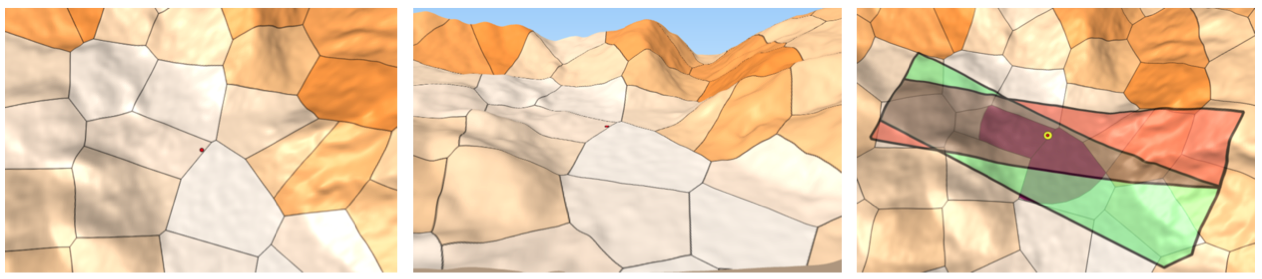
\includegraphics[width=0.9\textwidth]{images/PopoliFinal}
	\caption{Stazione di Popoli - Vittorito. Partendo dalla prima immagine a sinistra  troviamo la vista dall'alto, di profilo e frontale.}
	\label{Popoli_Final}
\end{figure}

Nelle figure \ref{popolilandslide1} e \ref{popolilandslide2} sono rappresentate le $nz_{i,j}$, con le rispettive landslide evidenziate con dei rettangoli colorati con i contorni in nero. La diversa colorazione ha l'unico scopo di differenziare ulteriormente, esclusivamente a livello visivo, tra loro le landslides.


\begin{figure}[h]
	\hspace{0.1\linewidth}
	\begin{minipage}[t]{0.35\linewidth}
		\centering
		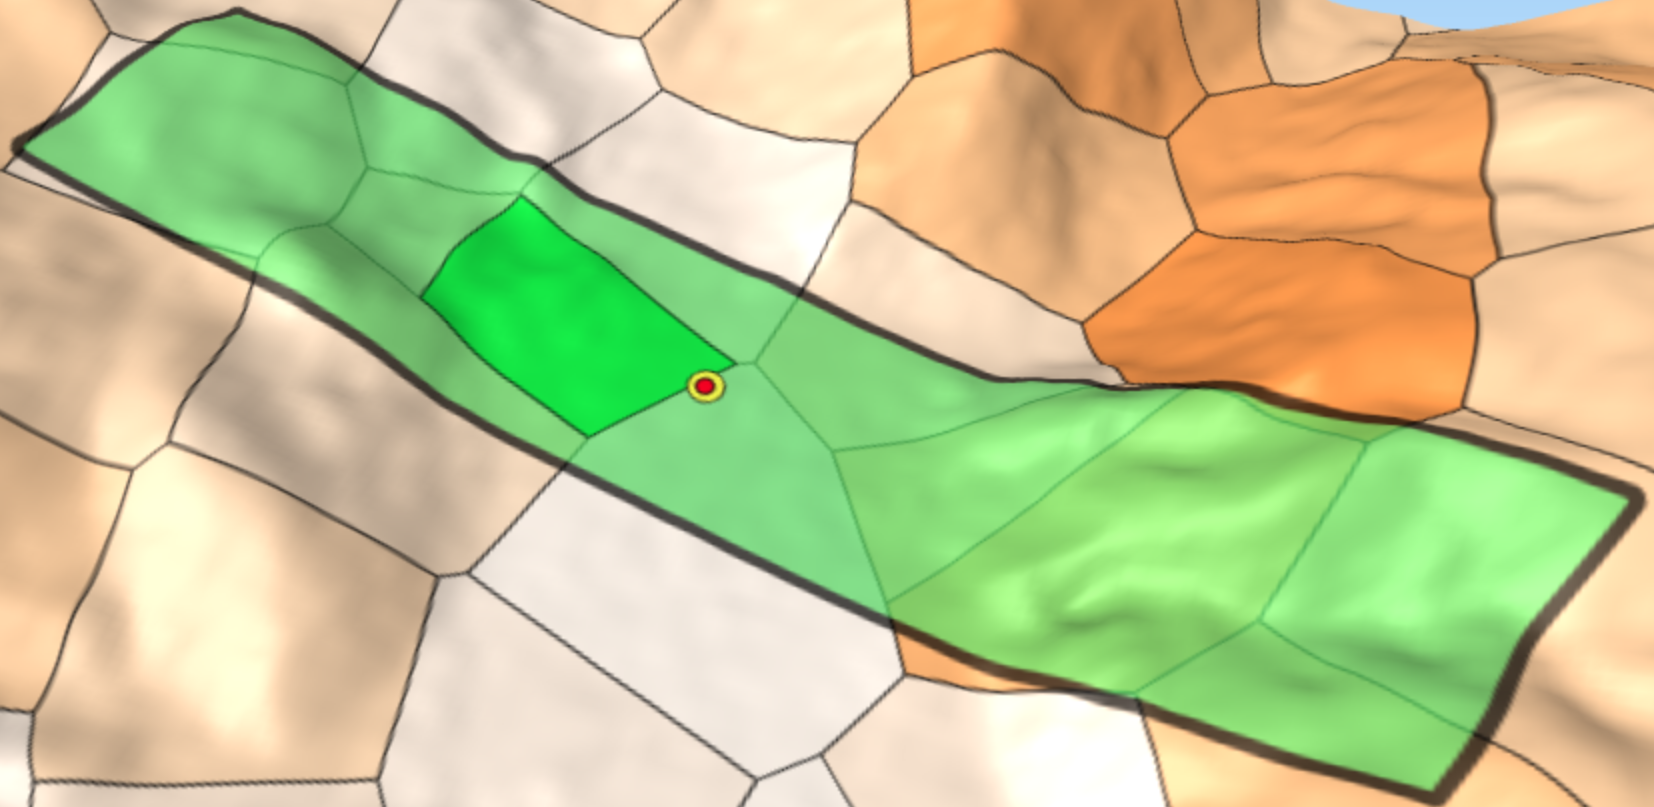
\includegraphics[width=1\textwidth]{images/PopoliLandslide1}
		\caption{La prima landslide della stazione di Popoli.}
		\label{popolilandslide1}
	\end{minipage}
	\hspace{0.1\linewidth}
	\begin{minipage}[t]{0.35\linewidth}
		\centering
		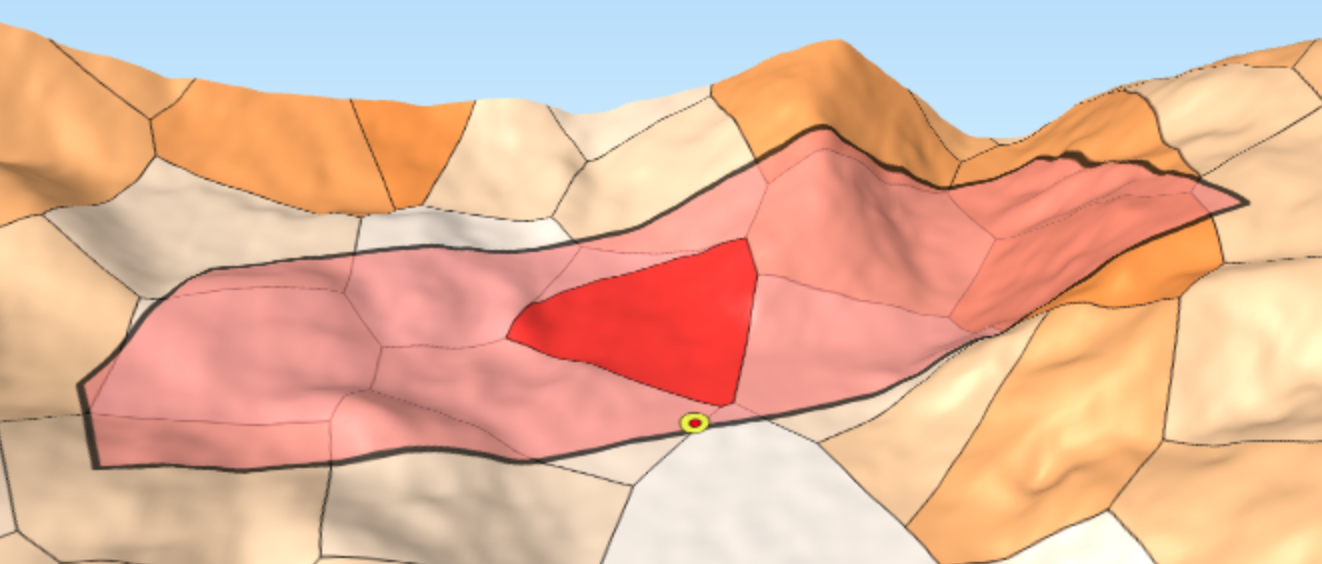
\includegraphics[width=1\textwidth]{images/PopoliLandslide2}
		\caption{La seconda ed ultima landslide della stazione di Popoli.}
		\label{popolilandslide2}
	\end{minipage}
\end{figure}


Apparentemente il metodo sembra funzionare correttamente, ma in realtà la landslide di colore verde ha una traiettoria inesatta. Come è possibile osservare in figura \ref{popolirect} le curve di livello all'interno della $nz_{i,j}$ seguono un percorso tortuoso.  Di conseguenza i centri di massa $czf_{i,j,t}$ delle zone fragments $zf_{i,j,t}$ non sono ben allineati ma sparsi nella $nz_{i,j}$. Questo comporta che l'interpolazione della retta è molto imprecisa in quanto alcuni $czf_{i,j,t}$ si trovano a distanze elevate rispetto alla retta di regressione lineare, ovvero il valore della somma degli scarti è alto. 

	\begin{figure}[h]
	\centering
	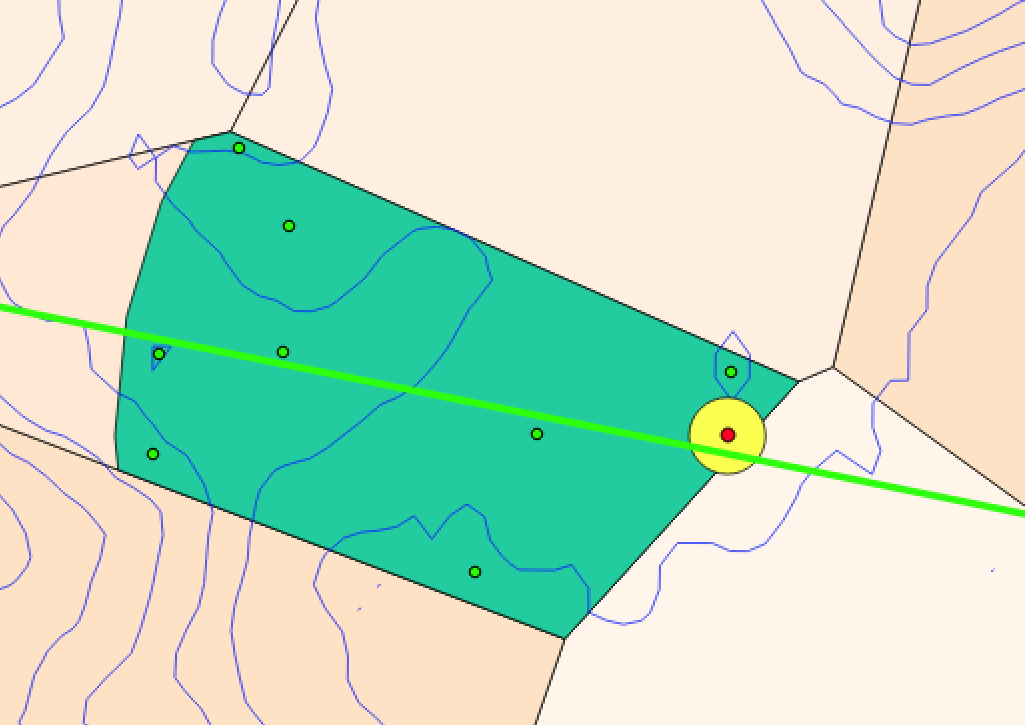
\includegraphics[width=0.5\textwidth]{images/PopoliRect}
	\caption{La retta di regressione lineare della prima landslide della stazione di Popoli.}
	\label{popolirect}
\end{figure}


In altre parole da questa nearest zone possono avere origine più landslides, come si evince dalla figura \ref{popolimultilandslide}. Dall'immagine ci si accorge che sulla stessa nearest zone ci sono diversi versanti di frana (almeno 4) evidenziati dalle frecce in rosso. Il metodo proposto non tiene conto di questo caso particolare e si comporta come se esistesse una sola frana. 

\begin{figure}[h]
	\centering
	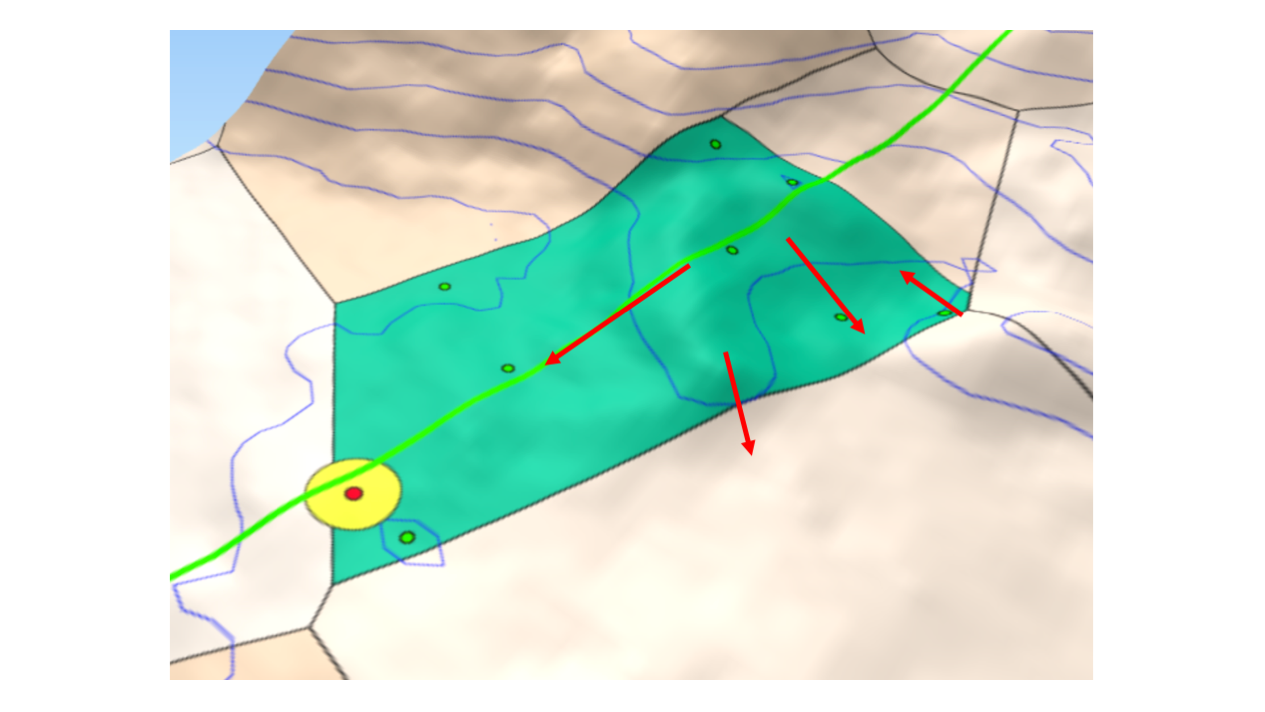
\includegraphics[width=0.6\textwidth]{images/PopoliMultiLandslide}
	\caption{Tutte le frane che potrebbero partire dalla nearest zone della landslide 1.}
	\label{popolimultilandslide}
\end{figure}

Per finire la landslide interseca il $BuildingBuffer_i$ e quindi contribuisce all'aumento dell'exposure della stazione. Ciò comporta il passaggio dalla classe bassa alla media e quindi ad una valutazione errata.

Il caso della stazione di Popoli - Vittorito evidenzia che il metodo proposto ha una limitazione che va presa in considerazione. Non è in grado di gestire più landslides che hanno origine dalla stessa nearest zone, ma per evitare questo inconveniente è sufficiente diminuire l'area delle zones.

\newpage 

\section{Stazione di Canistro}
La stazione di Canistro si trova in una vallata (Figura \ref{Canistro_Final}).  

	\begin{figure}[h]
	\centering
	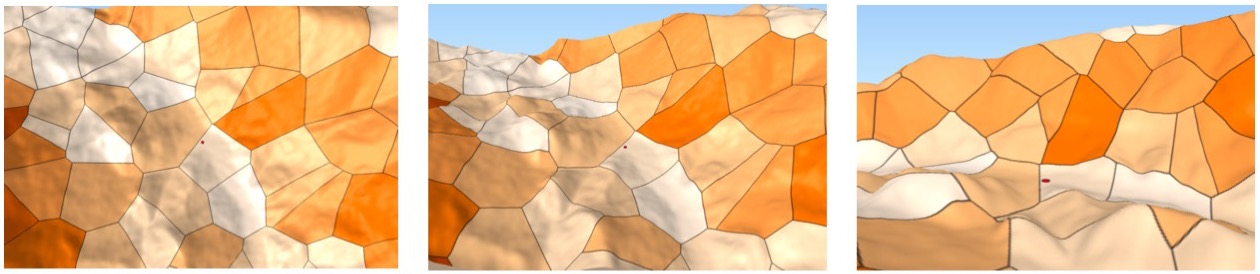
\includegraphics[width=0.9\textwidth]{images/CanistroFinal}
	\caption{Stazione di Canistro. Partendo dalla prima immagine a sinistra  troviamo la vista dall'alto, di profilo e frontale.}
	\label{Canistro_Final}
\end{figure}

Le landslides che impattano sulla stazione sono 4 (Figure \ref{canistrolandslide1}, \ref{canistrolandslide2}, \ref{canistrolandslide3}, \ref{canistrolandslide4}). 

\begin{figure}[h]
	\hspace{0.1\linewidth}
	\begin{minipage}[t]{0.35\linewidth}
		\centering
		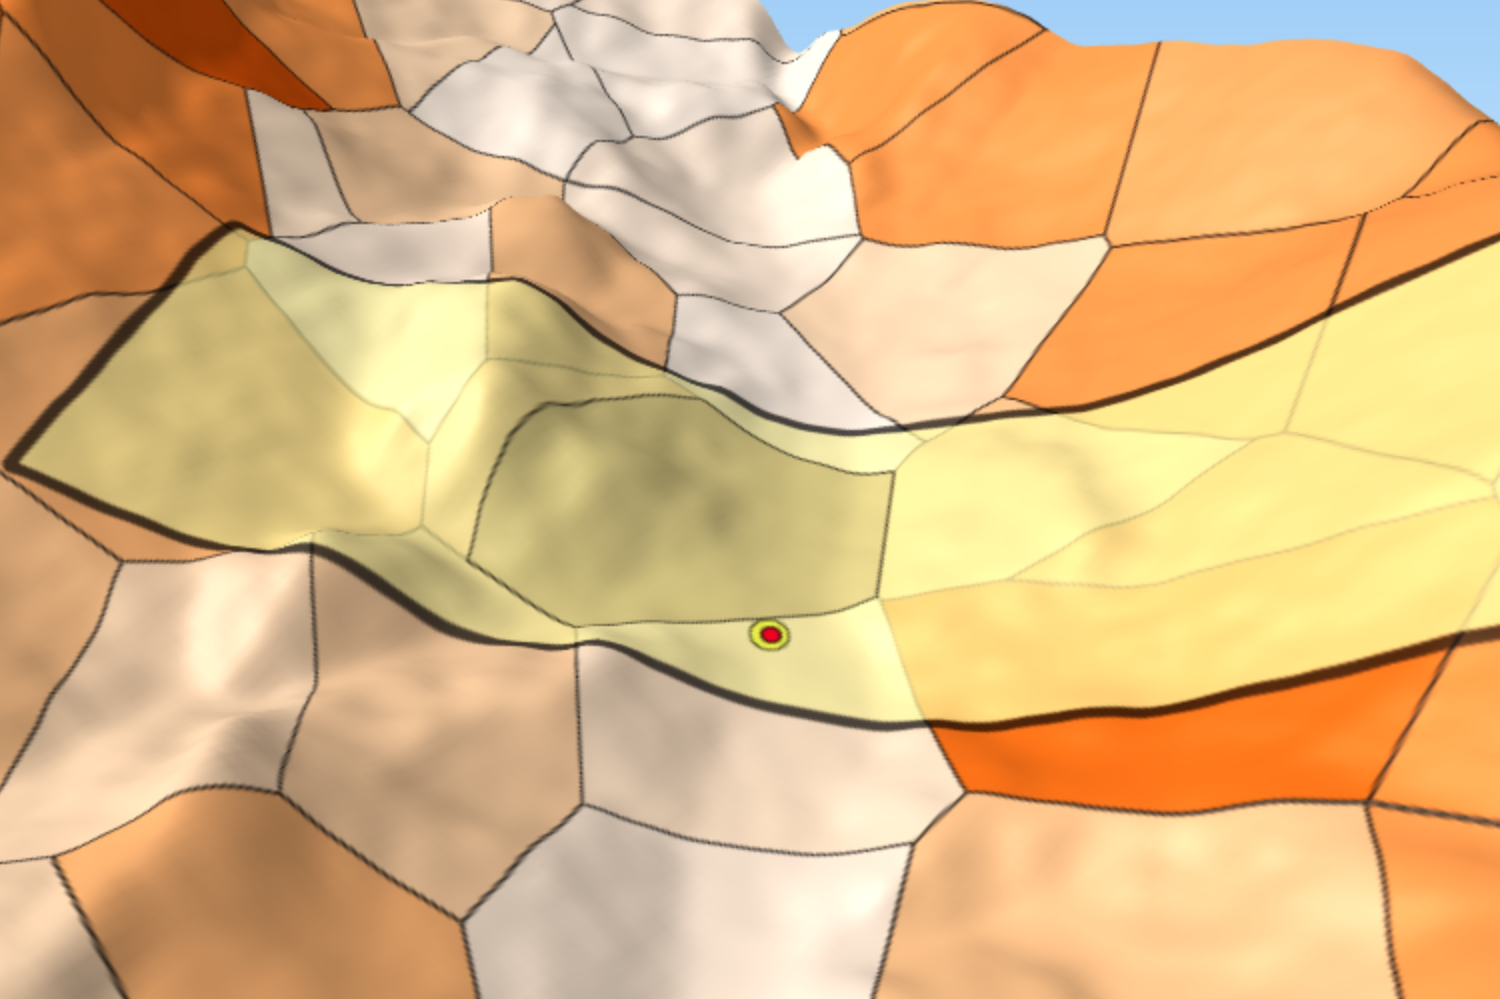
\includegraphics[width=1\textwidth]{images/CanistroLandslide1}
		\caption{La prima landslide della stazione di Canistro}
		\label{canistrolandslide1}
	\end{minipage}
	\hspace{0.1\linewidth}
	\begin{minipage}[t]{0.35\linewidth}
		\centering
		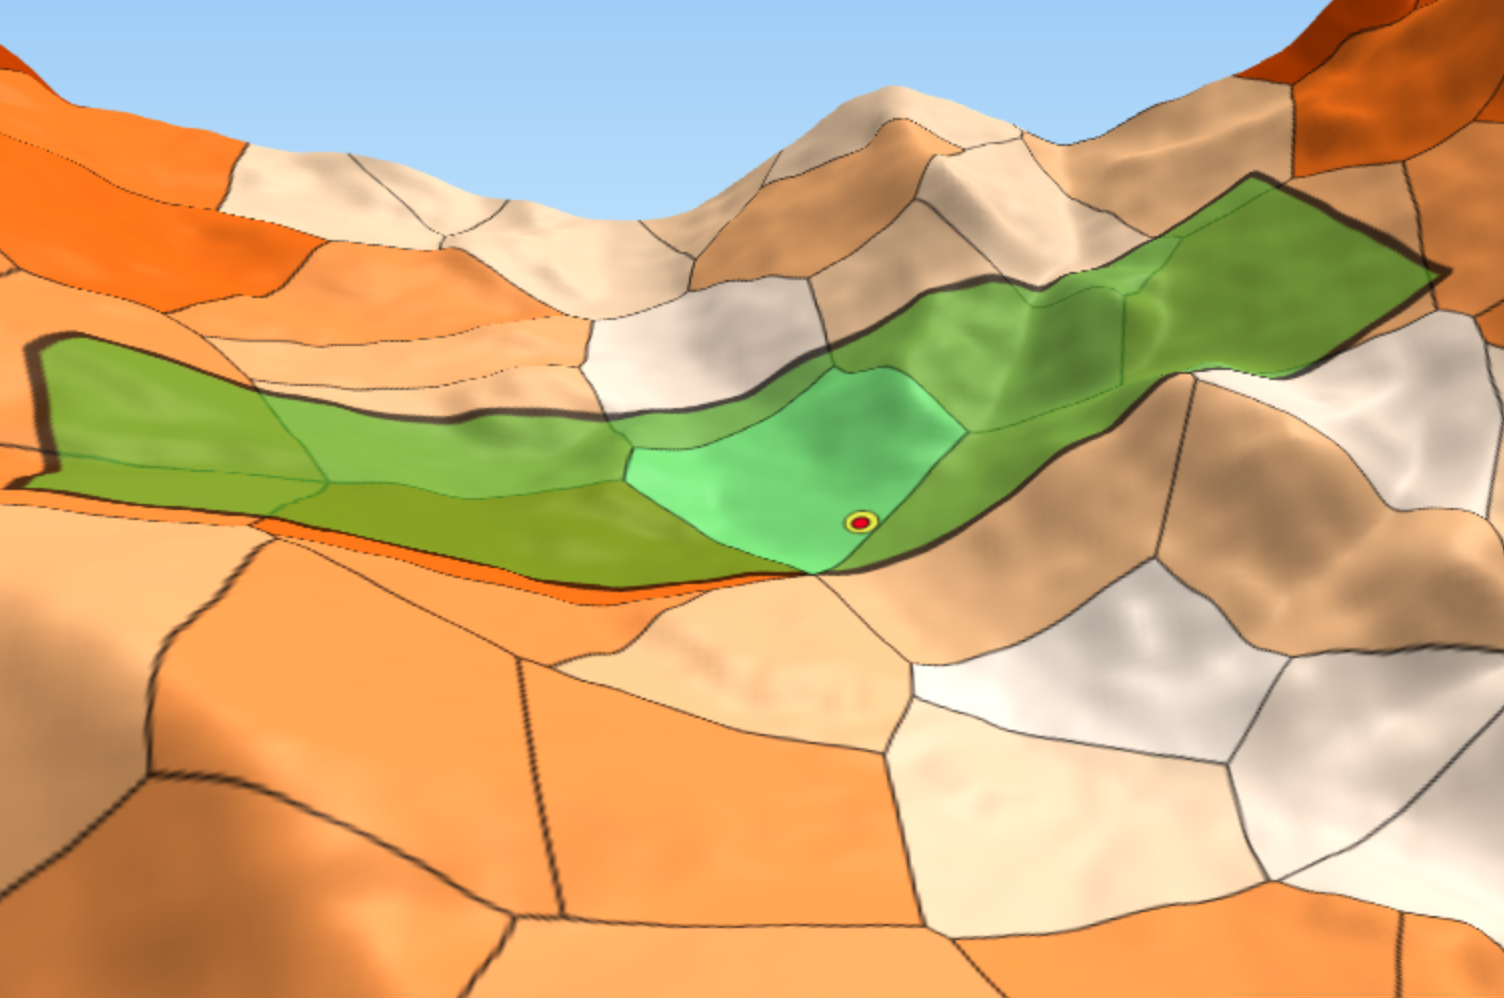
\includegraphics[width=1\textwidth]{images/CanistroLandslide2}
		\caption{La seconda landslide della stazione di Canistro}
		\label{canistrolandslide2}
	\end{minipage}
\end{figure}

\begin{figure}[h]
	\hspace{0.1\linewidth}
	\begin{minipage}[t]{0.35\linewidth}
		\centering
		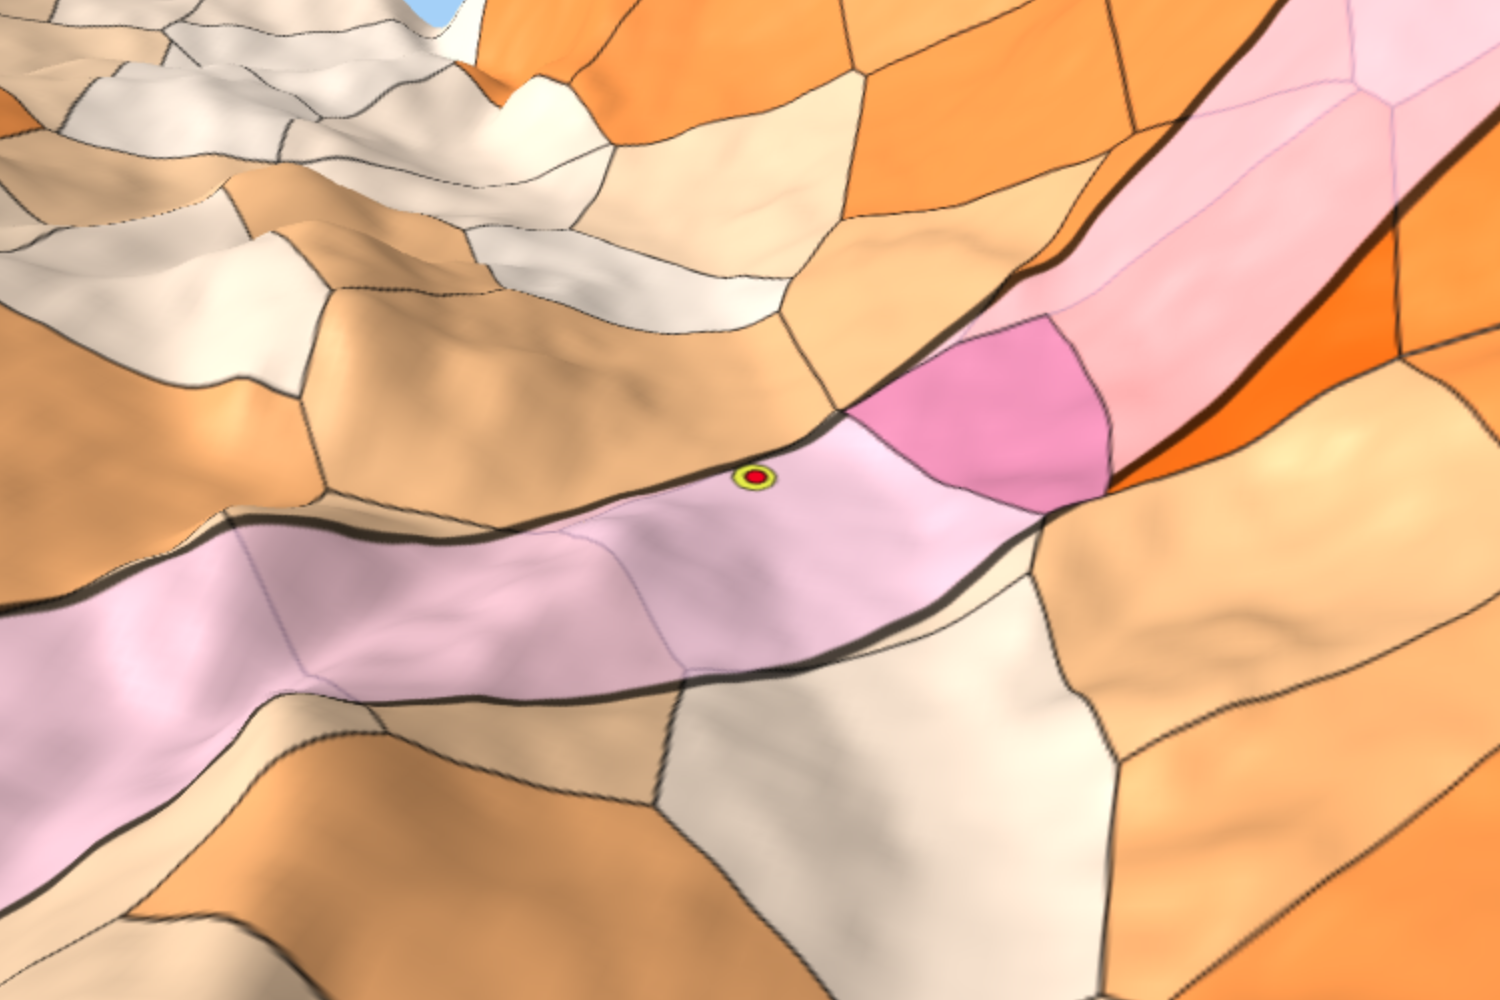
\includegraphics[width=1\textwidth]{images/CanistroLandslide3}
		\caption{La terza landslide della stazione di Canistro.}
		\label{canistrolandslide3}
	\end{minipage}
	\hspace{0.1\linewidth}
	\begin{minipage}[t]{0.35\linewidth}
		\centering
		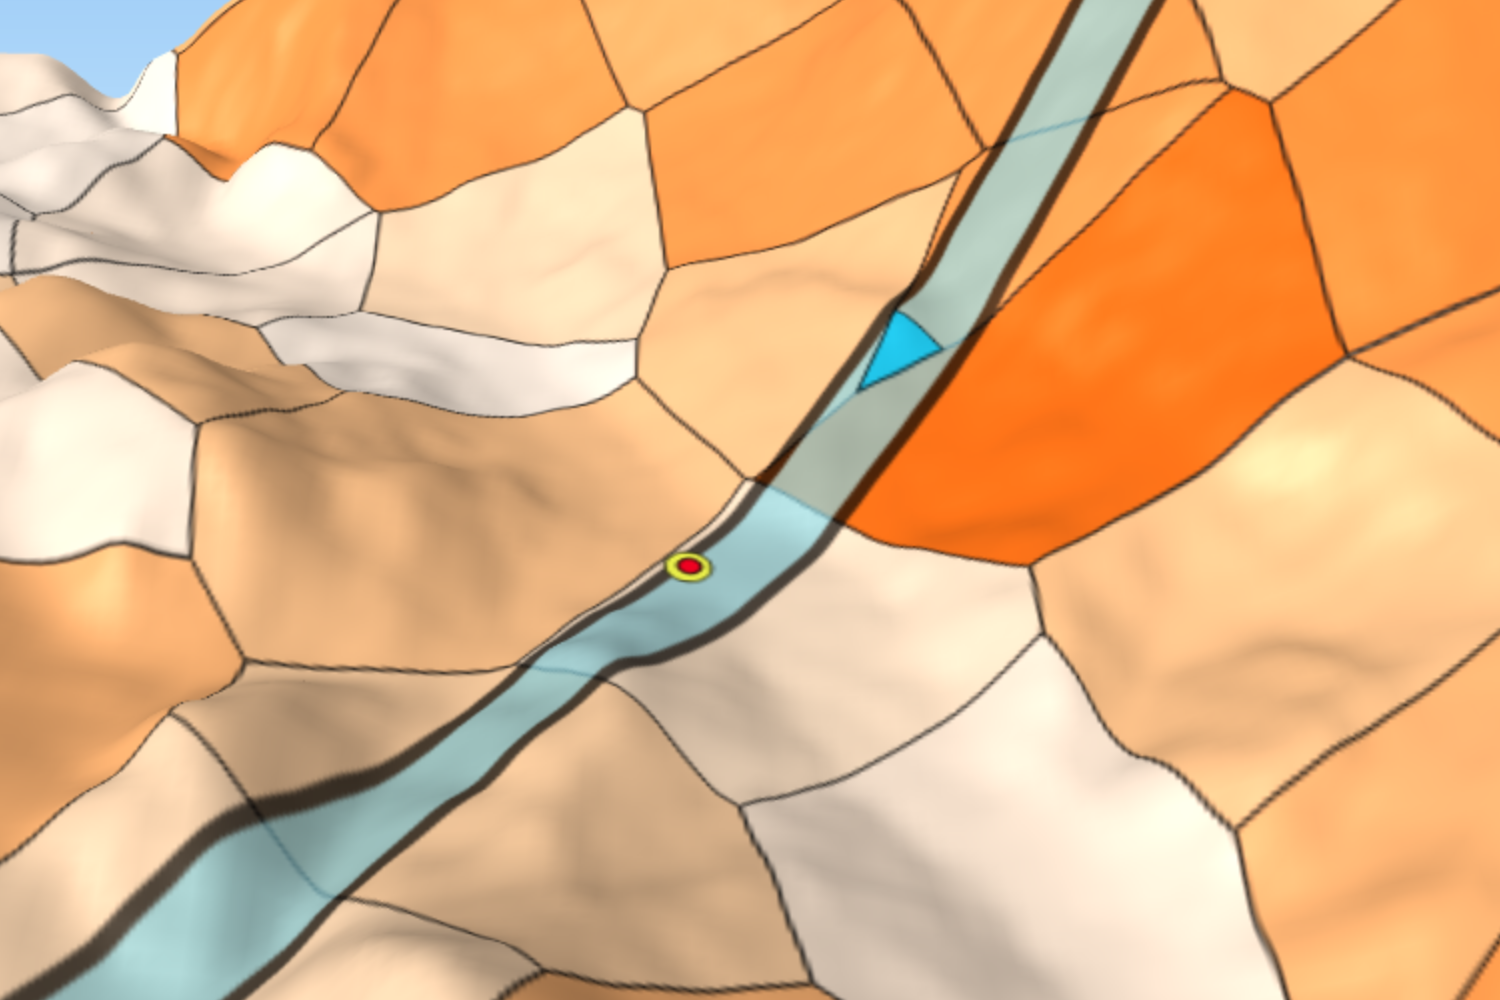
\includegraphics[width=1\textwidth]{images/CanistroLandslide4}
		\caption{La quarta ed ultima landslide della stazione di Canistro}
		\label{canistrolandslide4}
	\end{minipage}
\end{figure}


Due delle quali però non sono corrette. La landslide di colore verde è affetta dagli stessi problemi di traiettoria non corretta esaminati nella stazione precedente. Inoltre la landslide di colore giallo è troppo larga. Infatti nella figura \ref{wrongperimeter} è possibile vedere che la landslide è più larga dello $nz_{i,j}$ da cui parte.

\begin{figure}[h]
	\centering
	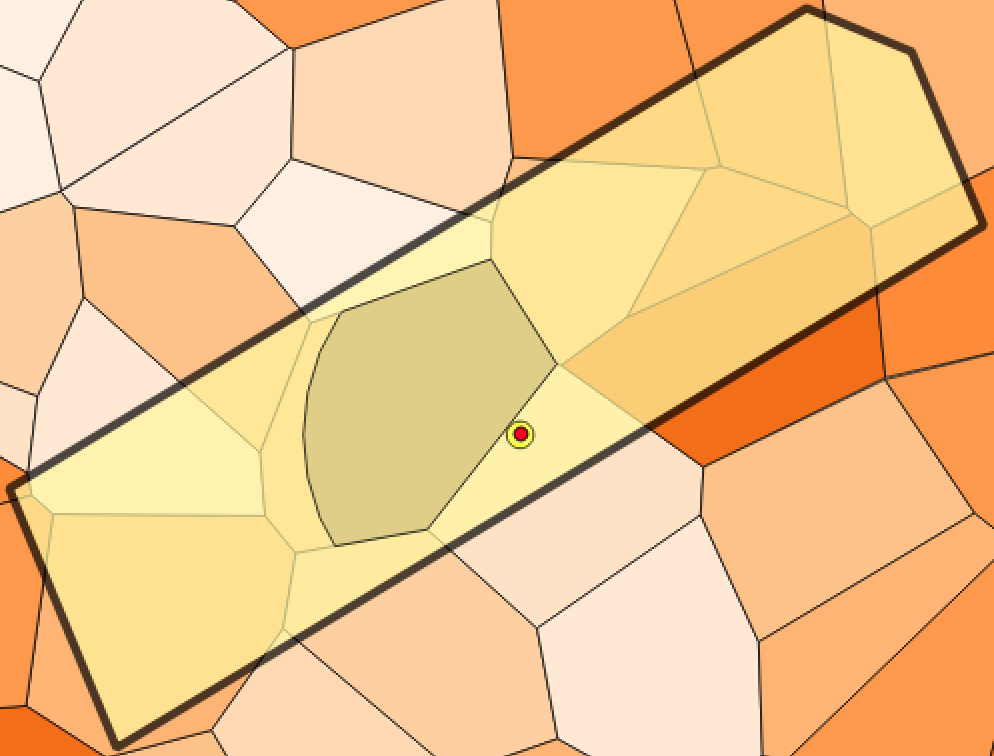
\includegraphics[width=0.5\textwidth]{images/WrongPerimeter}
	\caption{Landslide 1 vista dall'alto. }
	\label{wrongperimeter}
\end{figure}

Ciò accade perché la larghezza della landslide è proporzionata al perimetro della $nz_{i,j}$. Quest'ultima non è però di forma quadrata, ovvero non ha i lati tutti della stessa lunghezza. Per questo motivo bisognerebbe fare attenzione all'orientamento della landslide rispetto alla $nz_{i,j}$. In questo caso la landslide è  perpendicolare ai lati "corti" della $nz_{i,j}$. 

Ruotandola la landslide di 90 gradi in senso orario risulterebbe perpendicolare rispetto ai lati più lunghi e quindi la larghezza sarebbe corretta.

\begin{figure}[h]
	\centering
	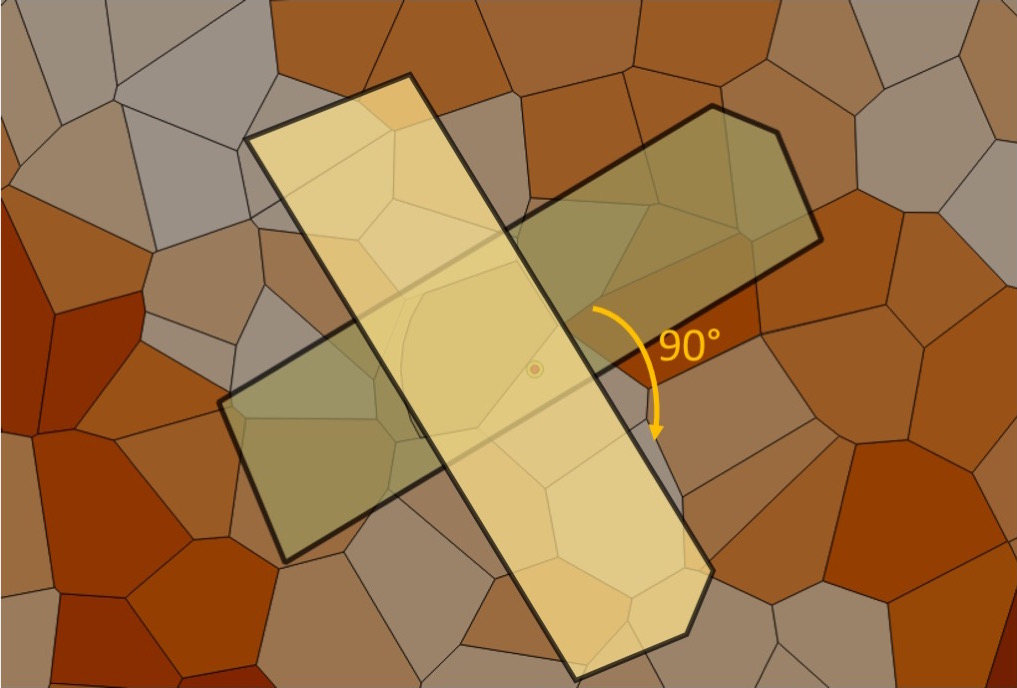
\includegraphics[width=0.6\textwidth]{images/LandslideRotation}
	\caption{La landslide 1 "ruotata" è larga quanto i lati lunghi della $nz_{i,j}$ da cui ha origine.}
	\label{landsliderotation}
\end{figure}


Questo aspetto ha una notevole rilevanza sull'equazione \ref{eq:impactfactor} dell'impact factor. Infatti l'area dell'intersezione tra il $BuildingBuffer_i$ e la landslide $ls_{i,j}$ risulta maggiorata, contribuendo all'aumento dell'exposure e di conseguenza ad una classificazione più alta.



\newpage
\section{Stazione di Fontecchio}
La stazione è molto vicina ai piedi di una montagna con pendii molto ripidi (Figura \ref{Fontecchio_Final}).  

	\begin{figure}[h]
	\centering
	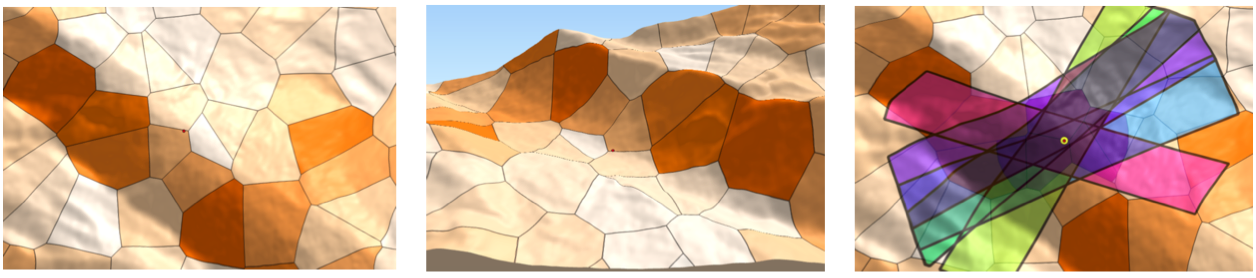
\includegraphics[width=0.9\textwidth]{images/FontecchioFinal}
	\caption{Stazione di Fontecchio. Partendo dalla prima immagine a sinistra  troviamo la vista dall'alto, di profilo e frontale.}
	\label{Fontecchio_Final}
\end{figure}

A differenza di Popoli-Vittorito e Canistro, la stazione di Fontecchio è un falso negativo che il metodo classifica con una classe più bassa rispetto a quella proposta dagli esperti. Le landslides che impattano sulla stazione sono 4 (Figure \ref{fontecchiolandslide1}, \ref{fontecchiolandslide2}, \ref{fontecchiolandslide3}, \ref{fontecchiolandslide4}).

	\begin{figure}[h]
	\hspace{0.1\linewidth}
	\begin{minipage}[t]{0.35\linewidth}
		\centering
		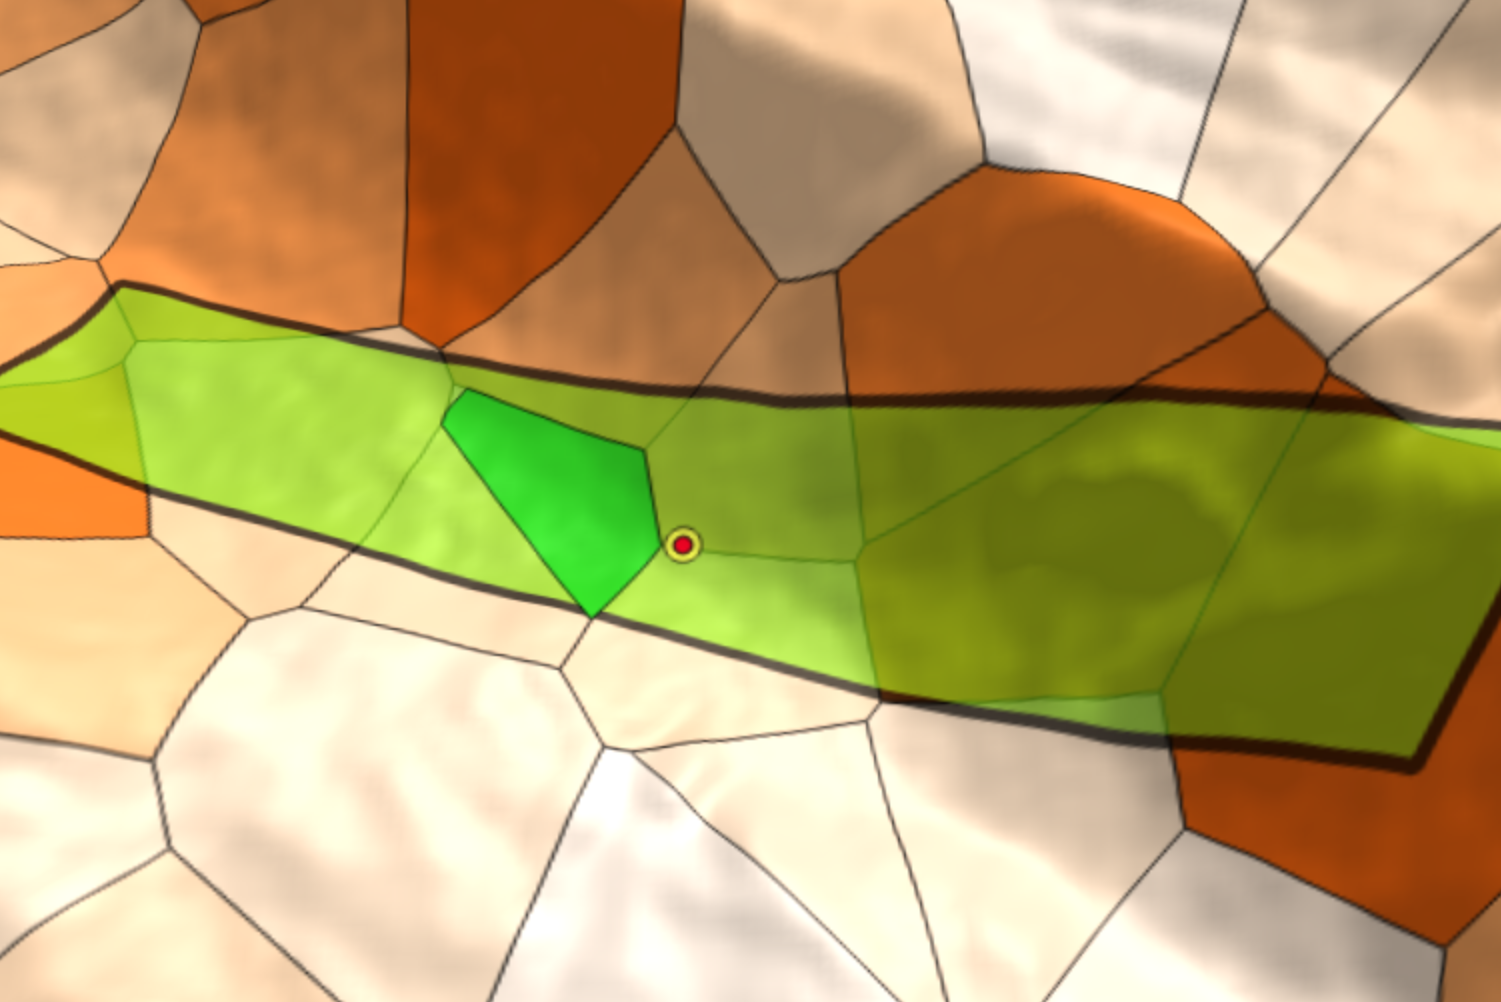
\includegraphics[width=1\textwidth]{images/FontecchioLandslide1}
		\caption{La prima landslide della stazione di Fontecchio.}
		\label{fontecchiolandslide1}
	\end{minipage}
	\hspace{0.1\linewidth}
	\begin{minipage}[t]{0.35\linewidth}
		\centering
		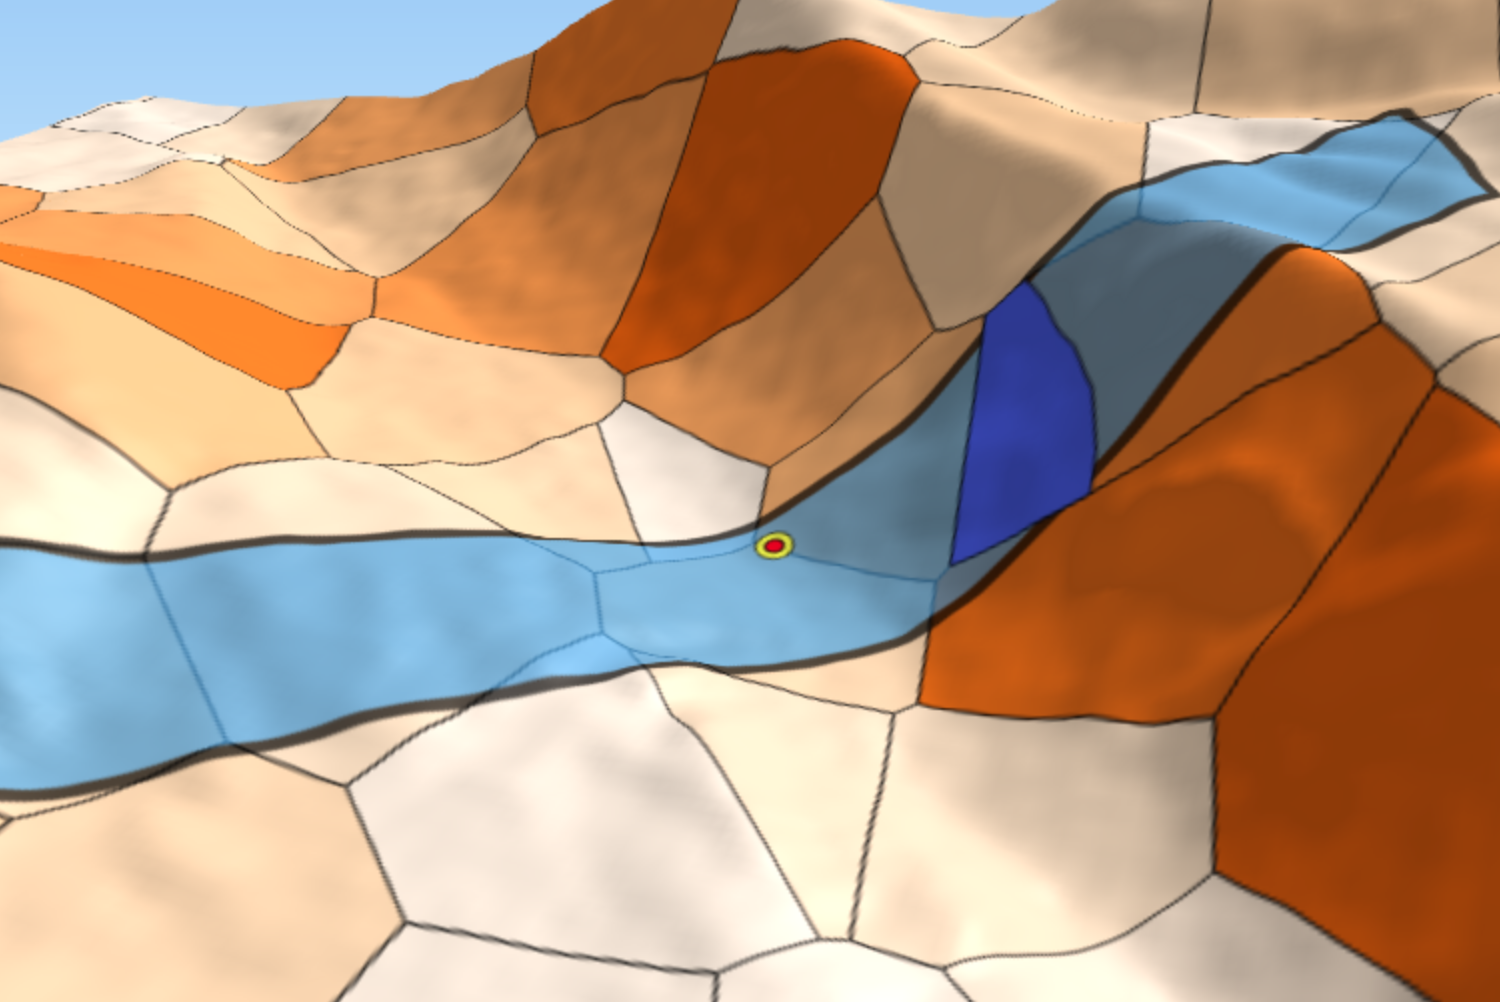
\includegraphics[width=1\textwidth]{images/FontecchioLandslide2}
		\caption{La seconda landslide della stazione di Fontecchio.}
		\label{fontecchiolandslide2}
	\end{minipage}
\end{figure}

\begin{figure}[h]
	\hspace{0.1\linewidth}
	\begin{minipage}[t]{0.35\linewidth}
		\centering
		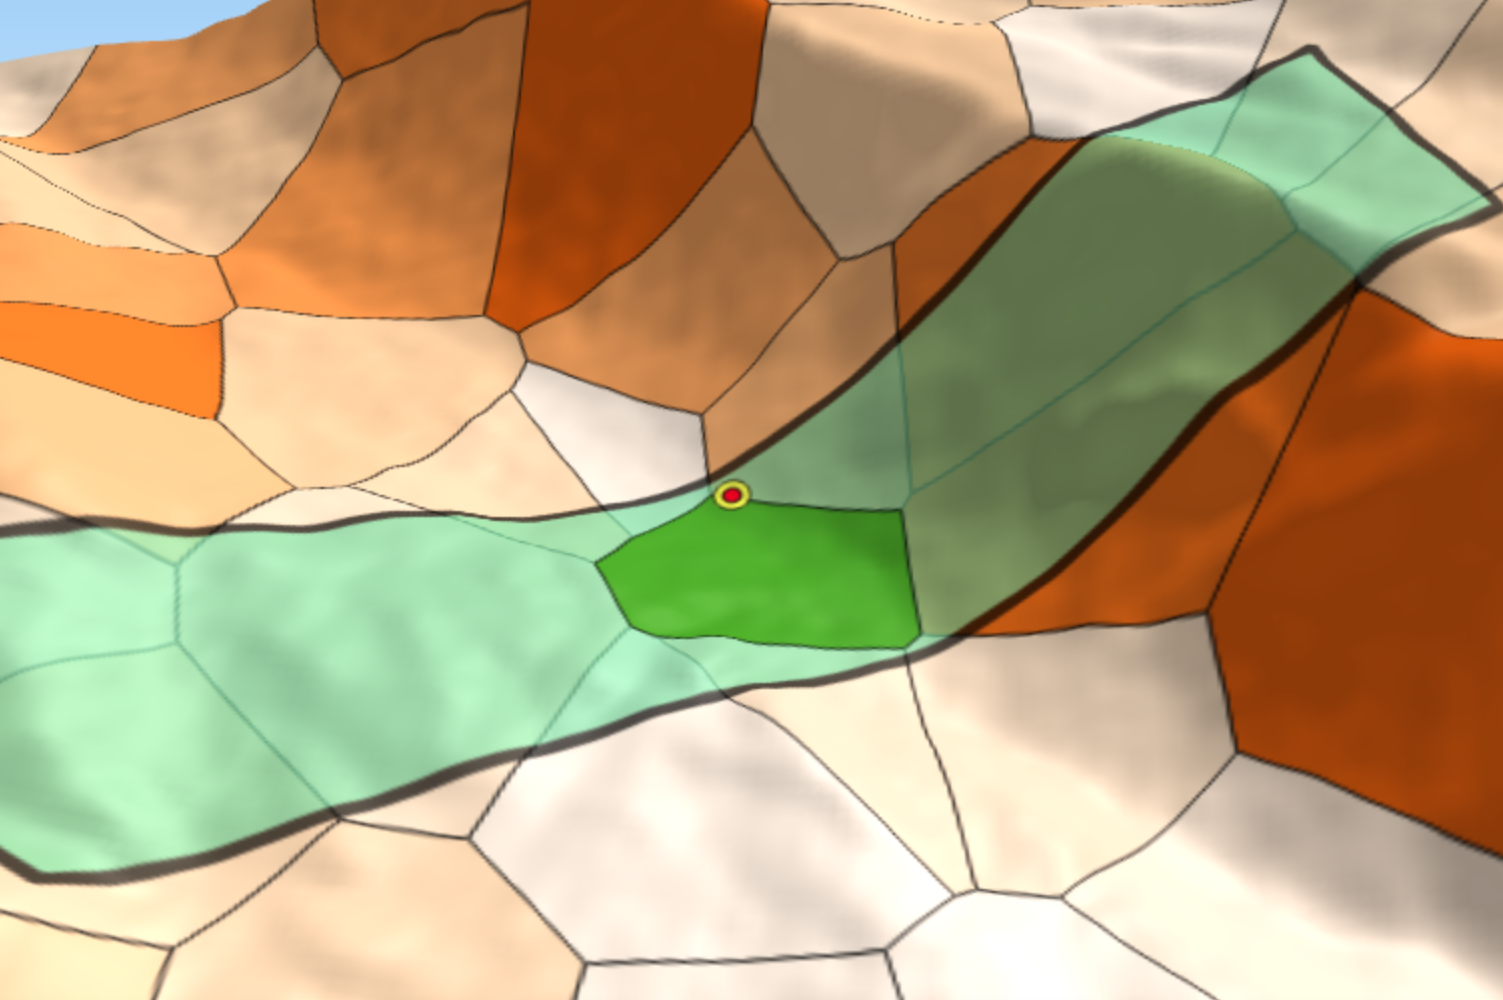
\includegraphics[width=1\textwidth]{images/FontecchioLandslide3}
		\caption{La terza landslide della stazione di Fontecchio.}
		\label{fontecchiolandslide3}
	\end{minipage}
	\hspace{0.1\linewidth}
	\begin{minipage}[t]{0.35\linewidth}
		\centering
		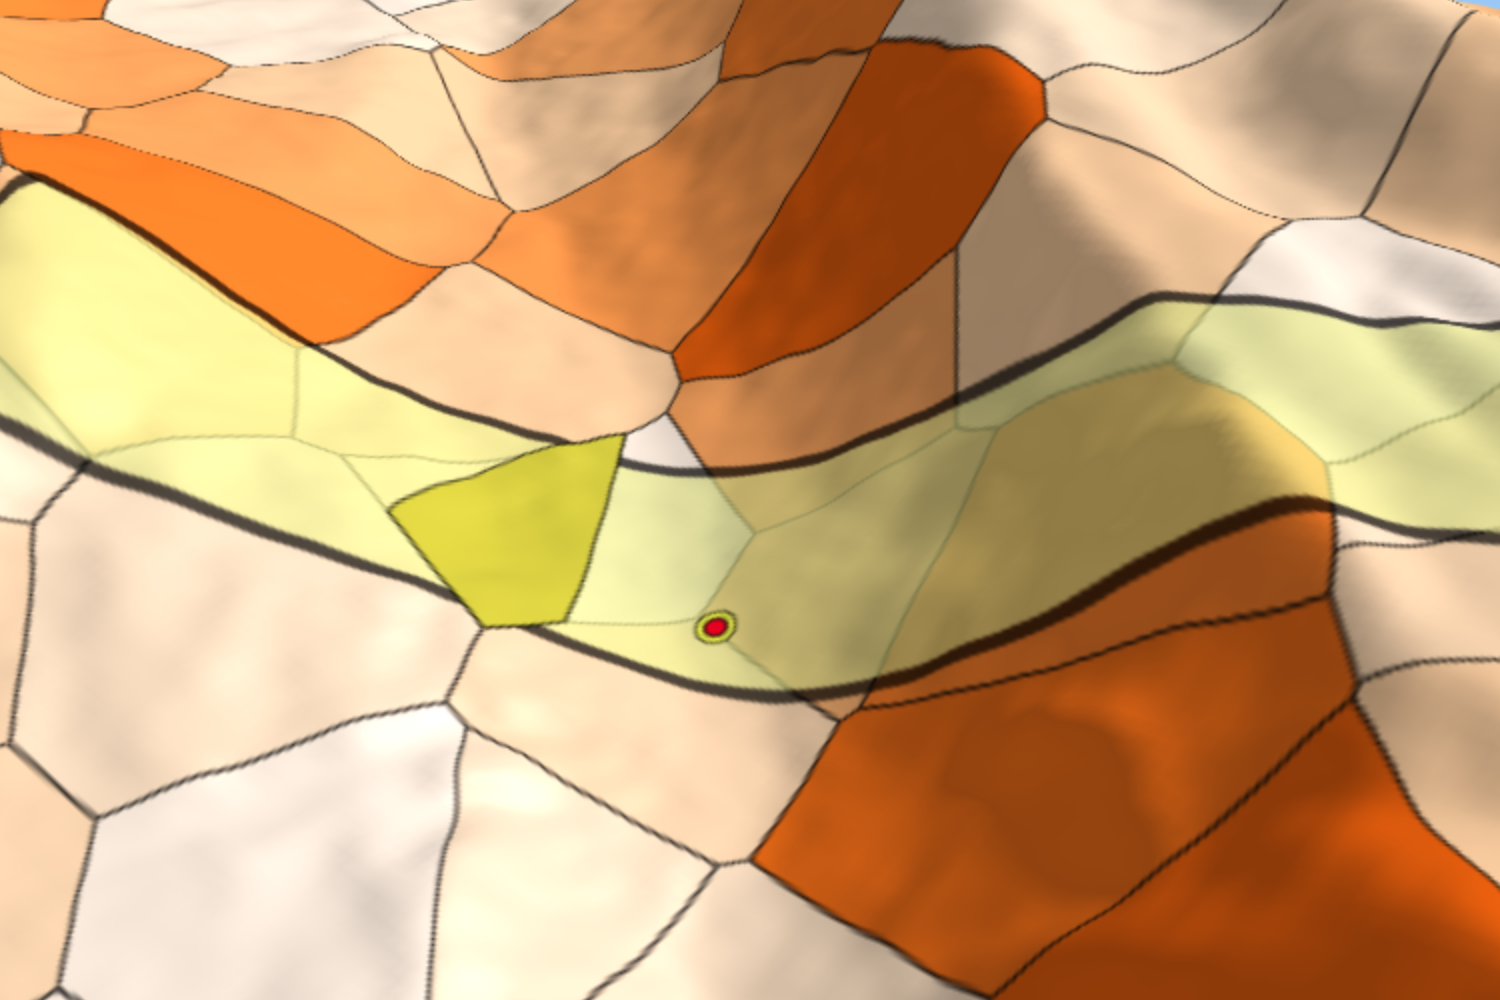
\includegraphics[width=1\textwidth]{images/FontecchioLandslide4}
		\caption{La quarta ed ultima landslide della stazione di Fontecchi.}
		\label{fontecchiolandslide4}
	\end{minipage}
\end{figure}

In questo caso le landslides hanno una traiettoria corretta. La landslide in figura \ref{fontecchiolandslide4} non contiene per intero la nearest zone da cui ha origine, motivo per cui dovrebbe avere una larghezza maggiore. Ciò nonostante, in questo caso, la landslide copre per intero il $BuildingBuffer_i$ e quindi il suo contributo all'exposure è corretto. A questo punto si può ricondurre la  classificazione errata all'insieme \textit{Z} in quanto gli $sz_k$ associati alle $nz_{i,j}$ hanno dei valori troppo bassi (Tabella \ref{tab:szk_fontecchio}). Infatti il valore medio degli è pari a 0.2949, che paragonato a quello delle  stazioni più ad alto rischio come  Sant'Ilario (0.3946), Aversa (0.4605) e Pettorano sul gizio (0.3739) è di gran lunga inferiore.

\begin{table}[h]
	\centering
	\caption{$Sz_k$ delle nearest zones della stazione di Fontecchio.}
	\label{tab:szk_fontecchio}
	\begin{tabular}{|l|c|c|}
		\hline
		\multicolumn{1}{|c|}{\cellcolor{gray!50} Id zone} & {\cellcolor{gray!50} $Sz_k$} \\ \hline
		8074 & 0.2081     \\ \hline
		8222  & 0.2158   \\ \hline
		2358 &  0.0885  \\ \hline
		8135  &  0.3689       \\ \hline
		7952  &  0.5936      \\ \hline
	\end{tabular}
\end{table}
